\documentclass[12pt, twoside]{article}
\usepackage[letterpaper, margin=1in, headsep=0.5in]{geometry}
\usepackage[english]{babel}
\usepackage[utf8]{inputenc}
\usepackage{amsmath}
\usepackage{amsfonts}
\usepackage{amssymb}
\usepackage{tikz}
%\usetikzlibrary{quotes, angles}

\usepackage{graphicx}
\usepackage{enumitem}
\usepackage{multicol}

\usepackage{fancyhdr}
\pagestyle{fancy}
\fancyhf{}
\renewcommand{\headrulewidth}{0pt} % disable the underline of the header

\fancyhead[LE]{\thepage}
\fancyhead[RO]{\thepage \\ Name: \hspace{4cm} \,\\}
\fancyhead[LO]{BECA / Dr. Huson / Geometry\\* Unit 7: Similarity\\* 6 January 2020}

\begin{document}
\subsubsection*{7.3 Do Now: Slope and the tangent function, similar triangles}
  \begin{enumerate}
  \item \begin{enumerate}[itemsep=1.5cm]
    \item Graph and label $\triangle ABC$ with $A(0,0)$, $B(4,7)$, and $C(4,0)$. Calculate each length:
    \begin{multicols}{2}
      \begin{enumerate}
        \item $AC=$
        \item $BC=$
        \item $AB=$ \vspace{3cm}
      \end{enumerate}
    \begin{center}
      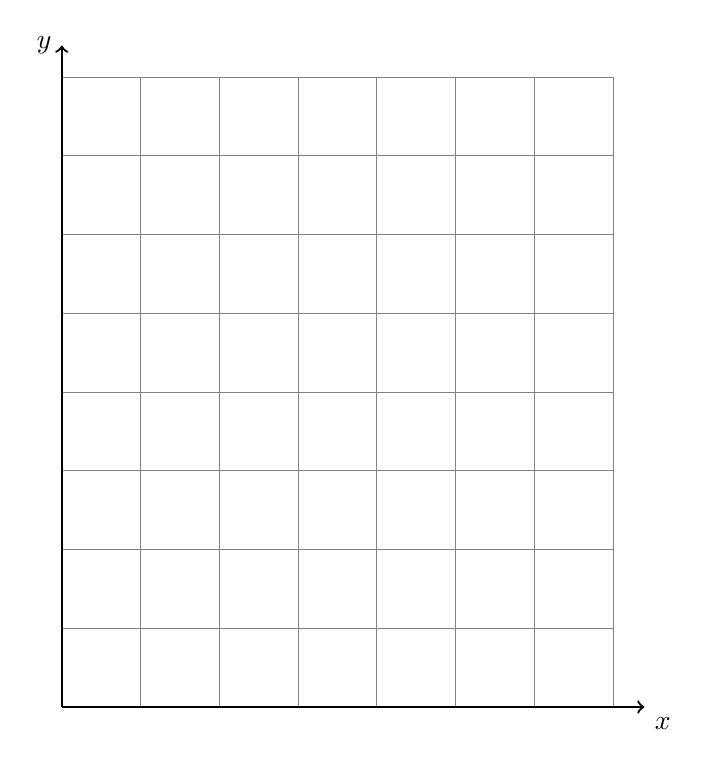
\begin{tikzpicture}%[scale=.635]
        \draw [help lines] (0,0) grid (7,8);
        \draw [thick, ->] (0,0) -- (7.4,0) node [below right] {$x$};
        \draw [thick, ->] (0,0)--(0,8.4) node [left] {$y$};
      \end{tikzpicture}
    \end{center}
  \end{multicols}%\vspace{2cm}
    \item Write down the equation of the line $\overleftrightarrow{BC}$.
    \item Write down the equation of the line $\overleftrightarrow{AB}$. 
    \item The tangent of an angle is the ratio of the side lengths \emph{opposite} over \emph{adjacent} to the angle. Write down the value as a fraction. \\[0.5cm]
      $\tan \angle BAC=$
    \item Find $m\angle BAC$ with a calculator's inverse tangent function, $\displaystyle m \angle BAC = \tan^{-1}(\frac{opp}{adj})$
    \vspace{2cm}
  \end{enumerate}

\newpage
  \item Express the result to the nearest thousandth.  \vspace{.5cm}
    \begin{multicols}{2}
      \begin{enumerate}
        \item $\tan 34^\circ = $ \vspace{1cm}
        \item $\tan 60^\circ =$
      \end{enumerate}
    \end{multicols} \vspace{1cm}

    \item Round each value to the nearest degree.  \vspace{.5cm}
    \begin{multicols}{2}
      \begin{enumerate}
        \item $\tan^{-1} (1) = $ \vspace{1cm}
        \item $\tan^{-1} (\sqrt{3}) =$
      \end{enumerate}
    \end{multicols} \vspace{1cm}

  \item Given right $\triangle JKL$ with $\overline{JK} \perp \overline{KL}$, $JK=8$, $m\angle J=22^\circ$. (mark the diagram)
      \begin{enumerate}
        \item Let $x$ be the length of the side opposite $\angle J$, $x=KL$. Write an equation expressing $\tan \angle J$ as a ratio of \emph{opposite} over \emph{adjacent}.  
      \begin{flushright}
          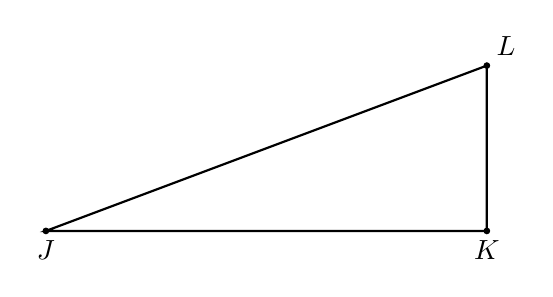
\begin{tikzpicture}[scale=0.7]
            \draw [thick](-1,0)--(7,0)--(7,3)--cycle;
            \draw [fill] (-1,0) circle [radius=0.05] node[below]{$J$};
            \draw [fill] (7,0) circle [radius=0.05] node[below]{$K$};
            \draw [fill] (7,3) circle [radius=0.05] node[above right]{$L$};
          \end{tikzpicture}
        \end{flushright}
        \item Solve the equation for $x=KL$. \vspace{3cm}
        \item Use the Pythagorean formula to find the length $JL$
      \end{enumerate}

\end{enumerate}
\end{document}